%
% main.tex -- Paper zum Thema <planet>
%
% (c) 2020 Autor, OST Ostschweizer Fachhochschule
%
% !TEX root = ../../buch.tex
% !TEX encoding = UTF-8
%
\chapter{Warum sind Planeten Sphären?\label{chapter:planet}}
\kopflinks{Warum sind Planeten Sphären?}
\begin{refsection}
\chapterauthor{Jakob Gierer und Lukas Schöpf}
\index{Jakob Gierer}%
\index{Gierer, Jakob}%
\index{Lukas Schöpf}%
\index{Schöpf, Lukas}%

%
% 0_Einleitung.tex
%
% (c) 2020 Prof Dr Andreas Müller, Hochschule Rapperswil
%
% !TEX root = ../../buch.tex
% !TEX encoding = UTF-8
%
\section{Einleitung\label{planet:section:einleitung}}
\rhead{Einleitung}
Was ist eigentlich ein Planet?
Wie unterscheidet man einen Planet von einem Zwergplaneten?
Genau diese Fragen stellten sich Wissenschaftler im Jahr 2006 \cite{planet:iaub5}.
Die Definition sieht folgendermassen aus.
Ein Planet ist ein Himmelskörper welcher:
\begin{enumerate}
	\item einen Orbit um eine Sonne hat,
	\item ausreichende Masse hat, damit seine Eigengravitation die Kräfte eines starren Körpers überwinden kann, sodass es eine hydrostatische Gleichgewichtsform (nahezu rund) annimmt, und
	\item die Umgebung seiner Umlaufbahn freigeräumt hat.
\end{enumerate}

\noindent
In diesem Kapitel wird die hydrostatische Gleichgewichtsform behandelt.
Sie wird in 2D und in 3D hergeleitet.



%
% teil1.tex -- Beispiel-File für das Paper
%
% (c) 2020 Prof Dr Andreas Müller, Hochschule Rapperswil
%
% !TEX root = ../../buch.tex
% !TEX encoding = UTF-8
%
\section{Herleitung hydrostatische Gleichgewichtsform
\label{planet:section:teil1}}
\rhead{Problemstellung}
Damit die hydrostatische Gleichgewichtsform einfacher berechnet werden kann, werden ein paar Annahmen getroffen.
\begin{itemize}
	\item Unser Himmelskörper besteht aus einer idealen Flüssigkeit, das heisst sie ist Inkompressibel und hat keine innere Reibung.
	\item Die Massenverteilungsdichte \(\sigma\) für 2D und die Dichte \(\rho\) für 3D der Flüssigkeit sind konstant.
	Dies ist eine Idealisierung der Bedingung 2 für die Definition eines Planeten.
\end{itemize}

Konkret sieht unsere Problemstellung folgendermassen aus.
\begin{itemize}
	\item Die potenzielle Energie \(U\) soll minimal werden.
	\item Die Fläche \(A\) bzw. das Volumen \(V\) ist gegeben.
	\item Da man eine runde Form erwartet, werden die Berechnungen in Polarkoordinaten bzw. Kugelkoordinaten durchgeführt. Somit suchen wir die Funktion \(r(\varphi)\) in 2D und \(r(\varphi,\theta)\) in 3D.
\end{itemize}

\subsection{Gravitation}

Die Kraft, welche Teilchen auf andere Teilchen ausüben, nennt man Gravitation.
Sie ist eine der vier Grundkräfte der Physik.
Die Gravitation kann man sich als Feld vorstellen.
Für die Berechnung der Kraft, welche auf ein Teilchen im Gravitationsfeld wirkt, benötigt man das Gravitationspotential \(\Phi\).
Es ist definiert als
\begin{equation}
	\Phi(r) = -\frac{GM}{r}.
	\label{planet:equ:gravpot}
\end{equation}
\(G\) ist die Gravitationskonstante \((G \approx 6.6743 \cdot 10^{-11} \text{m}^3 \text{kg}^{-1} \text{s}^{-2})\).
\(M\) ist die Masse des Körpers, welcher das Gravitationsfeld erzeugt, \(r\) der Abstand vom Ursprung.

Damit man die Kraft, welche auf ein Teilchen wirkt, berechnen kann, benötigt man den Gradienten des Gravitaionspotenzials, welcher definiert ist als
\begin{equation*}
	\nabla \Phi (r) = \frac{\partial \Phi}{\partial r} = \frac{\partial}{\partial r} \biggl( -\frac{GM}{r} \biggr) = \frac{GM}{r^2}.
\end{equation*}

Um nun die Kraft auf ein Teilchen zu berechnen muss man den Gradient des Gravitationspotenzials mit der Masse des Teilchens multiplizieren.
Somit lautet die Formel für die Berechnung der Kraft welche auf ein Teilchen wirkt
\begin{equation*}
	F = -m\nabla \Phi = -\frac{GMm}{\vec{r}^2}.
\end{equation*}
Die Kraft ist negativ, da sie zum Zentrum der Masse zeigen muss.


\subsection{Hydrostatische Gleichgewichtsform in 2D}
\begin{figure}
	\centering
	\includegraphics{papers/planet/pictures/Flächenelement.pdf}
	\caption{Visualisierung Polarkoordinaten}
	\label{planet:fig:2d}
\end{figure}
Für die Berechnung der hydrostatische Gleichgewichtsform soll nun die potenzielle Energie \(U\) minimal werden.
Für die Berechnung der Fläche in 2D muss man wissen, dass \(dA = r \, dr \, d\varphi\).
Dies sieht man in Abbildung \ref{planet:fig:2d}.
Als Nebenbedingung hat man die Fläche \(A\), welche mit 
\begin{equation}
	A = \int_{A}^{} dA
	\label{planet:equ:A}
\end{equation}
berechnet wird.
Die Formel für die Berechung der potenziellen Energie ist
\begin{equation}
	U = \int_{A} \sigma \, \Phi (r) \, dA.
	\label{planet:equ:U}
\end{equation}
Wenn man nun Gleichung \eqref{planet:equ:gravpot} in Gleichung \eqref{planet:equ:U} ein erhält man
\begin{equation*}
	U = \int_{0}^{2\pi}\int_{0}^{r(\varphi)} \frac{-GM}{r} \, \sigma r \, dr \, d\varphi.
\end{equation*}
Das erste Integral kann man auflösen und die Konstante aus dem Integral heraus nehmen, es resultiert 
\begin{equation}
	U =-GM\sigma \int_{0}^{2\pi} r(\varphi) \, d\varphi .
\end{equation}
Aus dieser Gleichung entnimmt man die Lagrange-Funktion
\begin{equation}
	L(\varphi ,r,r' = r(\varphi).
\end{equation}
Für die zweite Lagrange-Funktion schreiben wir die Gleichung der Nebenbedingung \eqref{planet:equ:A} aus zu
\begin{equation*}
	A = \int_{0}^{2\pi}\int_{0}^{r(\varphi)} r \, dr \, d\varphi.
\end{equation*}
Das innere Integral kann man auflösen, sodass die Gleichung zu
\begin{equation*}
	A = \int_{0}^{2\pi}\frac{r(\varphi)^2}{2} \, d\varphi
\end{equation*}
vereinfacht wird.
Aus diesem Integral entnimmt man die Lagrange-Funktion der Nebenbedingung
\begin{equation*}
	N(\varphi ,r,r' = \frac{r^2}{2}.
\end{equation*}

Um die gesuchte Lösung zu finden, nutzt man die Methode der Lagrange-Muliplikatoren.
Genaueres über die Methode der Lagrange-Muliplikatoren findet man in Kapitel \ref{buch:nebenbedingungen:lagrangemult:subsection:einzeln}.
Die wichtigsten Punkte, welche man für die Lösung dieser Problemstellung braucht, sind, dass man die Euler-Lagrange-Differentialgleichung als Gradienten ansehen kann.
Mit diesen Gradienten kann man anschliessend ein Gleichungssystem aufstellen und die gesuchte Funktion finden.
Damit man die gesuchte Funktion finden kann, muss man den Gradienten bzw. die Euler-Lagrange-Differentialgleichung der jeweiligen Lagrange-Funktionen berechnen und anschliessend in
\begin{equation}
	\nabla N \cdot \lambda = \nabla L
	\label{planet:equ:lamdagleichung}
\end{equation}
einsetzen.
Für den "'Gradienten"' der Lagrange-Funktionen benötigt man die jeweiligen partiellen Ableitungen
\begin{equation*}
	L(\varphi ,r(\varphi),r(\varphi)_\varphi) = r(\varphi),
	\frac{\partial L}{\partial r} = 1,
	\frac{\partial L}{\partial r'} = 0,
\end{equation*}
und
\begin{equation*}
	N(\varphi ,r(\varphi),r(\varphi)_\varphi) = \frac{r^2}{2} ,
	\frac{\partial N}{\partial r} = r,
	\frac{\partial N}{\partial r'} = 0.
\end{equation*}

Die "'Gradienten"' der Lagrange-Funktionen sind definiert als 
\begin{equation*}
	\nabla L = 
	\frac{\partial L}{\partial r}-  \frac{d}{d\varphi}\left( \frac{\partial L}{\partial r} \right)
\end{equation*}
und
\begin{equation*}
	\nabla N = \frac{\partial N}{\partial r} - \frac{d}{d\varphi}\left(\frac{\partial N}{\partial r'}\right).
\end{equation*}

Wenn man nun die Ableitungen der Lagrange-Funktionen in die "'Gradienten"' einsetzen
\begin{equation*}
	\left(\frac{\partial N}{\partial r} - \frac{d}{d\varphi}\left(\frac{\partial N}{\partial r'}\right)\right)\cdot \lambda = \frac{\partial L}{\partial r}-  \frac{d}{d\varphi}\left( \frac{\partial L}{\partial r'} \right)
\end{equation*} 
und anschliessend das Ganze in die Gleichung \eqref{planet:equ:lamdagleichung}
einsetzt und erhält man
\begin{equation*}
	r = \frac{1}{\lambda}.
\end{equation*}
Was sagt nun dieses Ergebnis?
Da \(\lambda\) ist eine Konstatnte muss \(r\) ebenfalls eine Konstante sein.
Da die Berechungen in Polarkoordinaten durchgeführt wurden, bedeutet ein konstanter Radius, dass die gesuchte Form ein Kreis ist.

\subsection{Hydrostatische Gleichgewichtsform in 3D}
\begin{figure}
	\centering
	\includegraphics{papers/planet/pictures/Flächenelement_spherical.pdf}
	\caption{Visualisierung Kugelkoordinaten}
	\label{planet:fig:3d}
\end{figure}
Für die Berechnung im 3-dimensionalen Raum geht man ähnlich vor wie im 2-dimensionalen Raum.
Der Unterschied ist, dass man eine weitere Variable \(\theta\) habt.
Da man nun mehr als eine Variable hat, muss man die Aufgabe mit der Euler-Ostrogadski-Differentialgleichung lösen.
Für die Berechnung der hydrostatische Gleichgewichtsform soll nun wieder die potenzielle Energie \(U\) minimal werden.
Da die Berechnungen in 3D durchgeführt werden, benötigt man für die Berechung die Formel für ein Volumenteilchen \(dV = r^2 \sin (\theta) \, dr \, d\theta \, d\varphi \).
Zu sehen ist dies in Abbildung \ref{planet:fig:3d}
Als Nebenbedingung hat man in 3D das Volumen \(V\) welches mit 
\begin{equation}
	V = \int_{V}^{} dV
	\label{planet:equ:V}
\end{equation}
berechnet wird.
Die Formel für die Berechnung der potenziellen Energie ist
\begin{equation}
	U = \int_{V} \sigma \,  \Phi (r)\, dV.
	\label{planet:equ:U3d}
\end{equation}
Nun setzt man wiederrum die Gleichung \eqref{planet:equ:gravpot} in Gleichung \eqref{planet:equ:U3d} erhält man
\begin{equation*}
	U = \int_{0}^{2\pi}
	\int_{0}^{\pi}
	\int_{0}^{r(\varphi,\theta)}
	\frac{-GM}{r}\, \sigma\, r^2 \sin (\theta) \,
	dr \, d\theta \, d\varphi.
\end{equation*}
Mit ein wenig Umstellen und dem Auflösen des ersten Integrals erhält man
\begin{equation*}
	U =-GM\sigma \int_{0}^{2\pi}\int_{0}^{\pi}\frac{r(\varphi,\theta)^2}{2}  \sin (\theta) \, d\theta \, d\varphi.
\end{equation*}
Wiederrum entnimmt man aus diesem Interal die Lagrange-Funktion
\begin{equation*}
	L(\varphi,\theta ,r,r_\varphi,r_\theta) = \frac{r^2}{2}  \sin (\theta).
\end{equation*}
Mit dem Wissen, dass \(dV = r^2 \sin (\theta) \, dr \, d\theta \, d\varphi \) kann man \eqref{planet:equ:V} als
\begin{equation*}
	V = \int_{0}^{2\pi}\int_{0}^{\pi}\int_{0}^{r(\varphi,\theta)} r^2 \sin (\theta) \, dr \, d\theta \, d\varphi
\end{equation*}
ausschreiben.
Hier löst man wiederrum das innere Integral, auf schreibt die Konstanten vor das Integral und erhält
\begin{equation*}
	V = \int_{0}^{2\pi}\int_{0}^{\pi}\frac{r(\varphi,\theta)^3}{3} \sin (\theta) \, d\theta \, d\varphi.
\end{equation*}
Aus dieser Gleichung entnimmt man die Lagrange-Funktion der Nebenbedingung
\begin{equation*}
	N(\varphi,\theta ,r,r_\varphi,r_\theta) = \frac{r^3}{3} \sin (\theta).
\end{equation*}
Wie in 2D findet man die gesuchte Funktion wenn man die Gleichung \eqref{planet:equ:lamdagleichung} löst.
Da man in der Berechung im 3D zwei Variablen hat (\(\varphi,\Theta\)), muss man die partiellen Ableitungen nach beiden Variablen berechnen.
Konkret benutzt man die Euler-Ostrogradski-Differentialgleichung als Gradient wenn die gesuchte Funktion von mehr als einer Varbiable abhängig ist.
Die Ableitungen sehen folgendermassen aus:
\begin{align*}
	\frac{\partial L}{\partial r} &= r  \sin (\theta) \\
	\frac{\partial L}{\partial r_\varphi} &= 0 \\
	\frac{\partial L}{\partial r_\theta} &= 0 \\
\intertext{und}
	\frac{\partial N}{\partial r} &= r^2\sin (\theta) \\
	\frac{\partial N}{\partial r_\varphi} &= 0 \\
	\frac{\partial N}{\partial r_\theta} &= 0
\end{align*}
Glücklicherweise werden viele der Ableitungen 0.
Die "'Gradienten"' sind definiert als
\begin{equation*}
	\nabla L =  \frac{\partial L}{\partial r} 
	-\frac{d}{d\varphi}\left( \frac{\partial L}{\partial r_\varphi} \right)
	-\frac{d}{d\theta}\left( \frac{\partial L}{\partial r_\theta} \right)
\end{equation*}
und
\begin{equation*}
	\nabla N=  \frac{\partial N}{\partial r} 
	-\frac{d}{d\varphi}\left( \frac{\partial N}{\partial r_\varphi} \right)
	-\frac{d}{d\theta}\left( \frac{\partial N}{\partial r_\theta} \right).
\end{equation*}
Somit können wir die "'Gradienten"' in die Gleichung \eqref{planet:equ:lamdagleichung} einsetzen und erhalten
\begin{equation*}
	r^2\sin (\theta) \cdot \lambda = r \sin (\theta).
\end{equation*}
Wenn man diese Gleichung weiter vereinfacht erhält man
\begin{equation*}
	r = \frac{1}{\lambda}.
\end{equation*}
Man sieht, das Ergebniss ist das selbe wie man in 2D erhält.
In 3D bedeutet ein Konstanter Radius, das die gesuchte Form eine Kugel ist.

\subsection{Interpretation der Ergebnisse}
Sowohl in 2D als auch in 3D erhält man das Ergebniss, dass die Form in welcher die potenzielle Energie eines Planeten minimiert wird, ein Kreis bzw. eine Kugel ist.
Diese Feststellung wird durch die Realität bestätigt, in der grössere Himmelskörper, welche ihre starren Körperkräfte überwinden, kugelähnliche Formen annehmen.


%
% 2_Multipol.tex
%
% (c) 2020 Prof Dr Andreas Müller, Hochschule Rapperswil
%
% !TEX root = ../../buch.tex
% !TEX encoding = UTF-8
%
\section{Multipolmoment
\label{planet:section:multipol}}
\rhead{Multipolmoment}
In der Physik ist die Multipolentwicklung ein Verfaheren um die Passion-Gleichung im Dreidimensionalen Raum zu lösen, die daraus entsteht eine Laurent-Reihe.
Die Entwicklungskoeffizienten dieser Reihe heissen Multipolmomente.
Diese Methode wird hauptsächlich in der Elektrostatik und Magnetostatik verwendet, kann aber auf jeder Gebiet der Physik verallgemeinert werden, in dem die Poisson-Gleichung vorhanden ist.

Die Motivation der Multipolentwicklung liegt darin, das Verhalten von beliebigen Potentialen (Gravitationspotential) in grosser Entfernung zu betrachten.

Dieser Abschnitt und die Herleitungen basieren auf den Inhalten von \cite{planet:multi} und \cite{planet:quadro}.

\begin{figure}[h!]
    \centering
    \includegraphics[width=\linewidth]{papers/planet/pictures/Multipol.pdf}
    \caption{Darstellung der Multipolentwicklung
        \label{planet:fig:multipol}}
\end{figure}

\subsection{Grundlagen
\label{planet:subsection:grundlagen}}

Die Poisson-Gleichung lässt sich allgemein als

\begin{equation*}
\Delta \phi (\vec{r}) = - f (\vec{r})
\end{equation*}

\noindent
schreiben, wobei \(\Delta\) der Laplace-Operator, \(f\) eine Dichte und \(\phi\) ein Potential ist (das Minus ist Konvention).
Die formale Lösung dieser Gleichung ist:

\begin{equation*}
\phi (\vec{r}) = \frac{1}{4\pi} \int d^3 \vec{r}\,' \frac{f (\vec{r}\,')} {\left| \vec{r} - \vec{r}\,' \right|}
\end{equation*}

\noindent
Ist \(f (\vec{r})\) in einem Volumen lokalisiert, kann für Orte \(\vec{r}\), die weit außerhalb dieses Volumens liegen, \(r \gg r\,'\), der Bruch in einer Taylor-Reihe in \(\vec{r}\,'\) um \(\vec{r}\,' = 0\) entwickelt werden:

\begin{equation*}
\frac{1}{\left| \vec{r} - \vec{r}\,' \right|} = \sum_{n=0}^{\infty} \frac{1}{n!} \left( \vec{r}\,' \cdot \vec{\nabla}\,' \right)^n \left. \frac{1}{\left| \vec{r} - \vec{r}\,' \right|} \right|_{\vec{r}\,'=0}
\end{equation*}

\noindent
Dabei bedeutet \(\vec{\nabla}\,'\), dass der Nablaoperator \(\vec{\nabla}\) nur auf die gestrichenen Koordinaten \(\vec{r}\,'\) und nicht auf \(\vec{r}\) wirkt.
Nach Bilden der Ableitungen wird diese an der Stelle \(\vec{r}\,' = 0\) ausgewertet.
Durch Umformen erhält man:

\begin{equation*}
\frac{1}{\left| \vec{r} - \vec{r}\,' \right|} = \sum_{n=0}^{\infty} \frac{1}{n!} \left( - \vec{r}\,' \cdot \vec{\nabla} \right)^n \frac{1}{r}
\end{equation*}

\noindent
Die genaue Form der Entwicklung und der Multipole hängt vom jeweiligen Koordinatensystem ab.

\subsection{Karthesische Multpolentwicklung
\label{planet:subsection:kartentwicklung}}

Die karthesische Multipolentwicklung wird im karthesischen Koordinatensystem durchgeführt.
Dort ist

\begin{equation*}
\vec{r}\,' \cdot \vec{\nabla} = r\,'_{i} \partial_{i},
\end{equation*}

\noindent
wobei Einsteinsche Summenkonvention verwendet wird.
Dann muss bei einem Summanden \(n\)-ter Ordnung ein Tensor \(n\)-ter Stufe, nämlich \(\textstyle \prod_{k=1}^{n} \partial_{i_{k}} \frac{1}{r}\) berechnet werden:

\begin{equation*}
\begin{aligned}
\frac{1}{\left| \vec{r} - \vec{r}\,' \right|} &= \frac{1}{r} - r\,'_{i} \partial_{i} \frac{1}{r} + \frac{1}{2} r\,'_{i} r\,'_{j} \partial_{i} \partial_{j} \frac{1}{r} + \mathcal{O}(r\,'^{3}) \\
&= \frac{1}{r} + r\,'_{i} \frac{r_{i}}{r^{3}} + \frac{1}{2} r\,'_{i} r\,'_{j} \frac{3 r_{i} r_{j} - r^{2} \delta_{ij}}{r^{5}} + \mathcal{O}(r\,'^{3}).
\end{aligned}
\end{equation*}

\noindent
Das Symbol \(\delta_{ij}\) repräsentiert das sogenannte Kronecker-Delta.
Die formale Lösung \(\phi (\vec{r})\) der Poisson-Gleichung ist unter Verwendung der Identität \(r\,'_{i} r\,'_{j} r^{2} \delta_{ij} = r\,'^{2} r_{i} r_{j} \delta_{ij}\) wie folgt darstellbar:

\begin{equation*}
\begin{aligned}
\phi (\vec{r}) &= \frac{1}{4\pi} \left[ \frac{1}{r} \underbrace{\int f (\vec{r}\,') \, d^3 \vec{r}\,'}_{\text{Monopol-}} + \frac{r_{i}}{r^{3}} \underbrace{\int d^3 \vec{r}\,' \, r\,'_{i} f (\vec{r}\,')}_{\text{Dipol-}} + \frac{1}{2} \frac{r_{i} r_{j}}{r^{5}} \underbrace{\int d^3 \vec{r}\,' \left( 3 r\,'_{i} r\,'_{j} - r\,'^{2} \delta_{ij} \right) f (\vec{r}\,')}_{\text{Quadrupolmoment}} + \dots \right] \\
&= \frac{1}{4\pi} \left[ \frac{1}{r} q + \frac{r_{i}}{r^{3}} p_{i} + \frac{1}{2} \frac{r_{i} r_{j}}{r^{5}} Q_{ij} + \dots \right]
\end{aligned}
\end{equation*}

In der entwickelten Reihe kommen die Faktoren \(r\) im Nenner mit steigendem Exponenten.
Dabei werden die höheren Ordnungen der Multipolmomente, mit zuhnemendem Abstand zum beobachteten Volumen immer weiter vernachlässigbar.
Es wurde einfachheitshalber für die Berechnungen der Kugelfrom in diesem Kapitel als Approximation das erste Moment verwendet und die höheren vernachlässigt.



\subsection{Anwendung
\label{planet:subsection:anwendung}}

Die Gravitation hat im Gegensatz zum Elekrtomagnetismus nur positive Ladungen, die Massen.
Es können dennoch gravitative Multipole definiert werden.
Aus der Poisson-Gleichung des Newtonschen Gravitationsgesetzes

\begin{equation}
    \Delta \Phi = -4\pi G\rho
\end{equation}

\noindent
Mit der Gravitationskonstante \(G\) und der Massendichte \(\rho\) ist der gravitative Monopol die Gesamtmasse \(M\).

Da Massen nur positiv sind lässt sich, aus den Ladungen kein Dipolmoment bilden.
Aus diesem Grund ist der gravitative Quadrupol nicht über zwei Dipole definiert.
Dennoch haben Massen verteilungen Quadrupole.
\cref{planet:fig:quadroearth} zeigt ein solches wobei, die blau gefärbten Abweichungen, das fehlen der Masse als negative Masse gesehen wird und die rot gefärbten Abweichungen, die überschüssigen Massen als positive Massen betrachtet wird.  

\begin{figure}[h!]
    \centering
    \includegraphics[width=\linewidth]{papers/planet/pictures/Quadroearth.pdf}
    \caption{Beispiel eines gravitativen Quadrupol
        \label{planet:fig:quadroearth}}
\end{figure}

\beispiel{Die Erde ist durch ihre Rotation keine perfekte Kugel, sie ist leicht eingedellt an den Polen und am Äquator bildet sich ein Wulst \cref{planet:fig:quadroearth}.
Desweiteren sind durch bestimmte Dichteunterschiede weitere Abweichungen der Kugelfrom, in \cref{geoid} ersichtlich.}

Einige himmelsmechanische Phänomene, wie die dynamische Entwicklung der Bahnelemente von Satelliten, lassen sich mit dem daraus resultierenden Quadrupolmoment beschreiben.

%
% 3_Arrokoth.tex
%
% (c) 2020 Prof Dr Andreas Müller, Hochschule Rapperswil
%
% !TEX root = ../../buch.tex
% !TEX encoding = UTF-8
%
\section{Arrokoth
\label{planet:section:arrokoth}}
\rhead{Arrokoth}

Arrokoth in \cref{planet:fig:arrokoth} ersichtlich, ist ein kleiner Asteroid aus dem Kuipergürtel, auch unter der ursprünglichen Bezeichnung (486958) 2014 MU69 sowie unter seinem Spitznamen Ultima Thule bekannt ist.
Der Name Arrokoth ist Powhatan/Algonquianisch und heisst „Himmel“.

Arrokoth ist das am weitesten entfernte Objekt, das jemals mit einer Raumsonde erforscht wurde.
Es wurde mit Hilfe des Hubble Weltraum Teleskopes 2014 vom New Horizions Wissenschaftsteam entdeckt.
Die Informationen zu Arrokoth sind von \cite{planet:arrokoth} entnommen.

Solche Weltraumschneemänner können nur entstehen wenn die eigene Gravitation kleiner ist als die starren Kräfte des Körpers.
Das bedeutet die Himmelskörper sind kleinere Objekte im Vergleich zu Planeten.
Zusätzlich dazu dürfen die einzelnen Asteroiden nicht mit grosser Kraft aufeinander treffen, das bedeutet verbinden der zwei Körper geschieht relativ langsam.
Wenn zwei Asteroiden mit grosser Geschwindigkeit aufeinander treffen, würden sie in kleinere Trümmer zerschmettert die über längeren Zeitraum wieder ein Asteroid bilden der widerum eine Kugelform hat.

\begin{figure}[h]
    \centering
    \includegraphics[width=\linewidth]{papers/planet/pictures/Arrokoth.pdf}
    \caption{Arrokoth aus dem Kuipergürtel \cite{planet:arrokothpic}
        \label{planet:fig:arrokoth}}
\end{figure}
%
% 4_Goce.tex
%
% (c) 2020 Prof Dr Andreas Müller, Hochschule Rapperswil
%
% !TEX root = ../../buch.tex
% !TEX encoding = UTF-8
%
\section{GOCE
\label{planet:section:goce}}
\rhead{GOCE}

Die folgenden Angaben zur GOCE-Mission in diesem Abschnitt stammen von \cite{planet:goce}.

\begin{figure}[h]
    \centering
    \includegraphics[width=\linewidth]{papers/planet/pictures/goce.pdf}
    \caption{Sattelit aus der GOCE Mission \cite{planet:gocepic}
        \label{planet:fig:goce}}
\end{figure}

Der Gravity Field and Steady-State Ocean Circulation Explorer (GOCE) ist ein Satellit, der im März 2009 von der Europäischen Weltraumorganisation ESA ins Weltall geschickt wurde.
GOCE umkreist die Erde in einer erdnahen Umlaufbahn von nur 260\,km Höhe, um das Schwerefeld der Erde mit bisher unerreichter Genauigkeit und räumlicher Auflösung zu erfassen.
Dafür nutzt GOCE einen Gradiometer unterstützt durch GPS um zusätzlich in Echtzeit die Navigation der Umlaufbahn aufzuzeichnen.

Das Gradiometer basiert auf drei Paare von Beschleunigungssensoren.
Das Gradiometer misst den Gradienten der Gravitation, um eine sehr genaue Erfassung des Geoid der Erde zu erstellen, in \cref{planet:fig:geoid} zu sehen.
Dies gibt einen Einblick in die inneren Strukturen der Erde, sowie in die Strömungen in den Tiefen der Ozeane.
Die zweite Funktion des Gradiometers besteht darin die Beschleunigung in Flugrichtung zu messen und den Schub von GOCE zu bestimmen, damit sich das Raumschiff nahezu im freien Fall befindet.

In der \cref{planet:fig:geoid} ist das Gravitationsfeld in den gelben Bereichen höher und in den blauen niedriger.
Aus dem \cref{planet:section:multipol} wird ersichtlich, was die Multipolentwicklung der Kugelform bedeutet, sie beschreibt die Abweichung von der perfekten Kugelform.
Die GOCE-Resultate werden daher mit den Multipolkoeffizienten geliefert.

\begin{figure}[h]
    \centering
    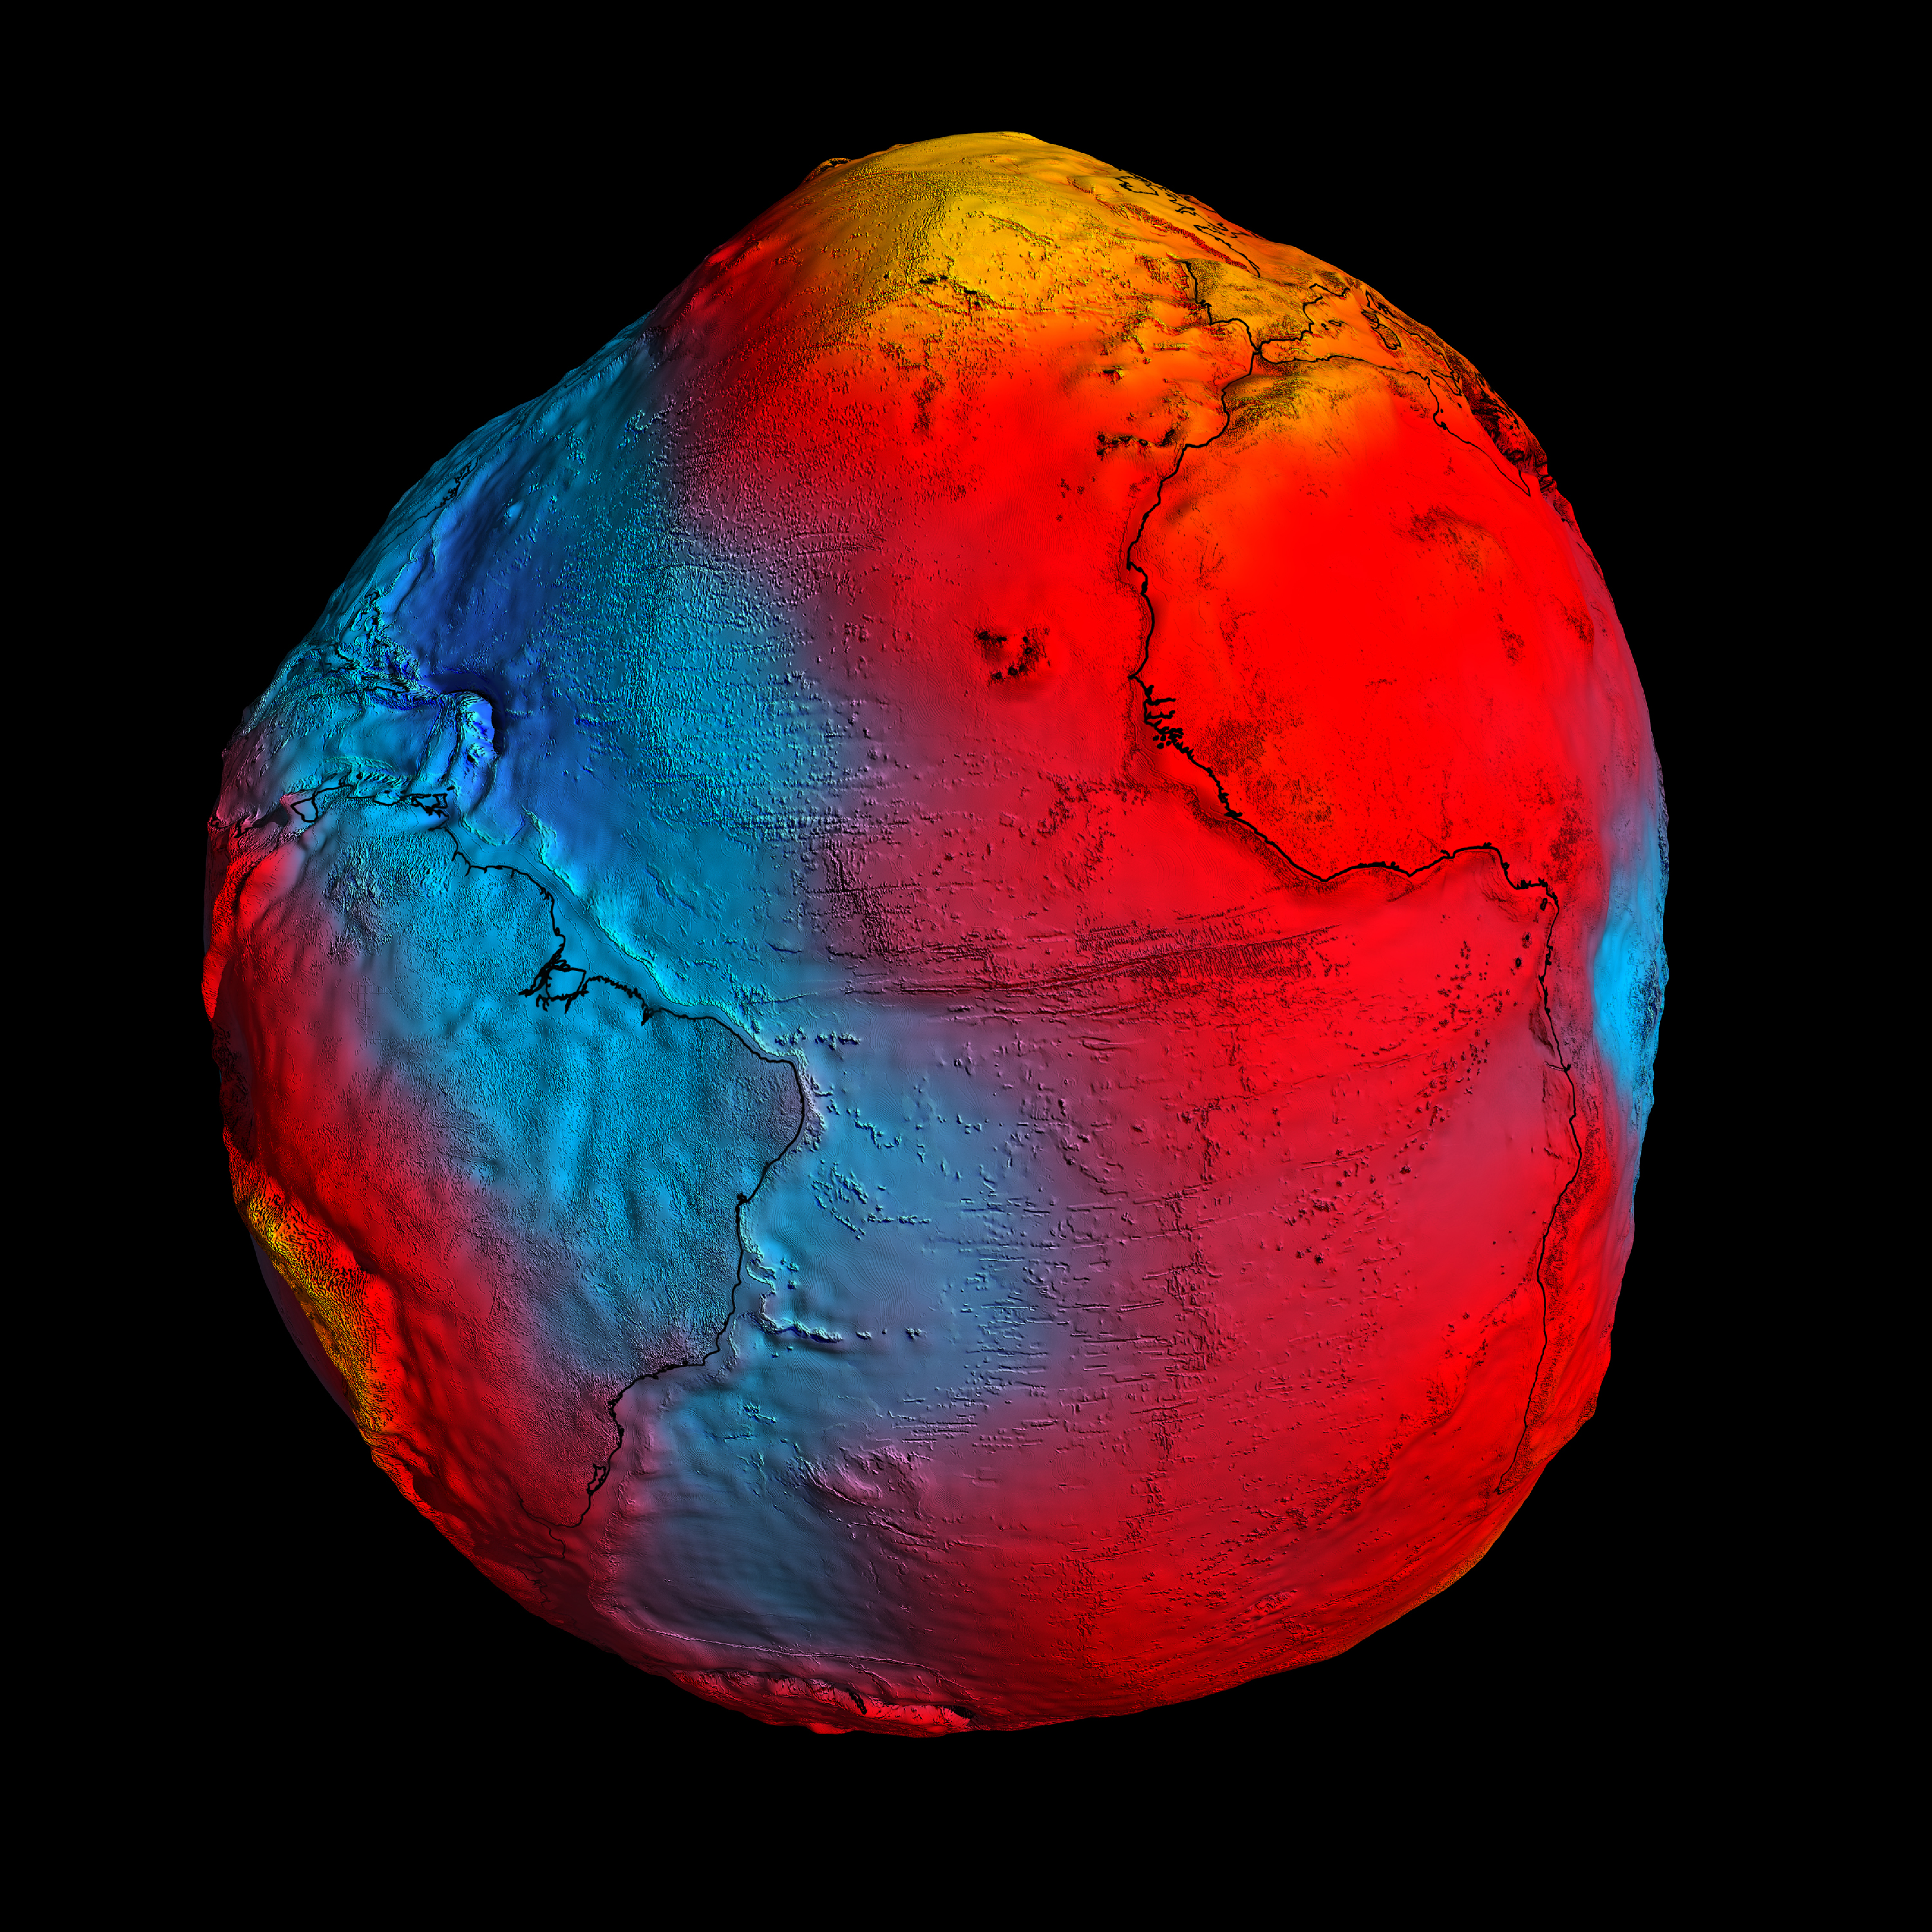
\includegraphics[width=\linewidth]{papers/planet/pictures/geoid.pdf}
    \caption{Darstellung des Gravitationsfelds der Erde \cite{planet:geoidpic}
        \label{planet:fig:geoid}}
\end{figure}




\printbibliography[heading=subbibliography]
\end{refsection}
